\chapter{Goals}

\section{Introduction}
Modern machine learning models based on deep neural networks are achieving remarkable performance on many fields, including medical image analysis. In comparison
with classic machine learning technologies like decision trees, it is much harder to explain how a neural network came to its conclusion, because it uses thousands to millions of training parameters.

In recent years, many methods for the interpretability of deep (convolutional) neural networks have been proposed, e.g. LIME\cite{ribeiro2016should}, RISE\cite{Petsiuk2018rise}, Grad-CAM\cite{selvaraju2017grad} or DeepLIFT \cite{shrikumar2017learning}.

\begin{figure}[h]
\centering
\caption{Examples of some interpreatbility methods for image classification \cite{visualattribution}}
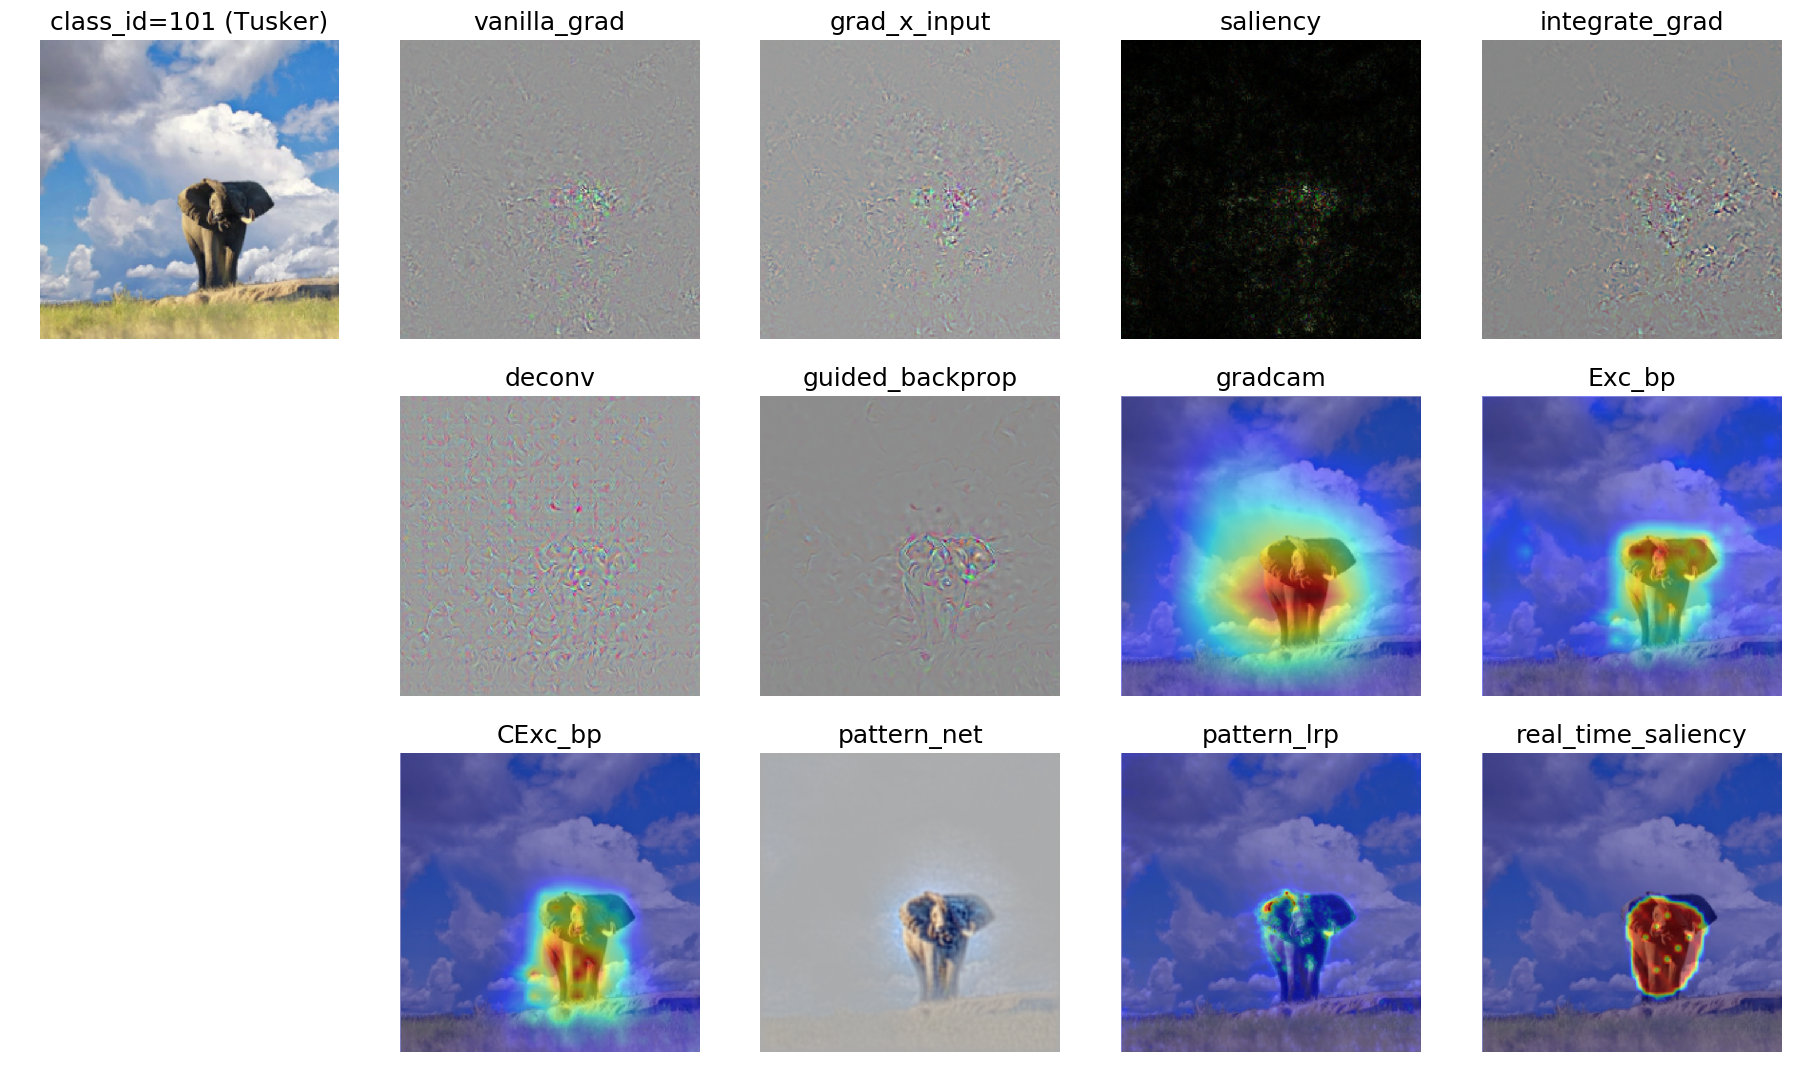
\includegraphics[width=14cm]{images/tusker_saliency.png}
\end{figure}

These methods focus on providing explanations and interpretability of classification problems for datasets like ImageNet or MNIST. What has not yet been researched much is the interpretability of image segmentation tasks. On many image segmentation tasks, interpretability based image regions like gradcam (see image above) does not make that much sense, because the segmentation already returns a region of an image.

\begin{figure}[H]
\centering
\caption{Image segmentation on MRI scans of the brain\cite{soltaninejad2017automated}}
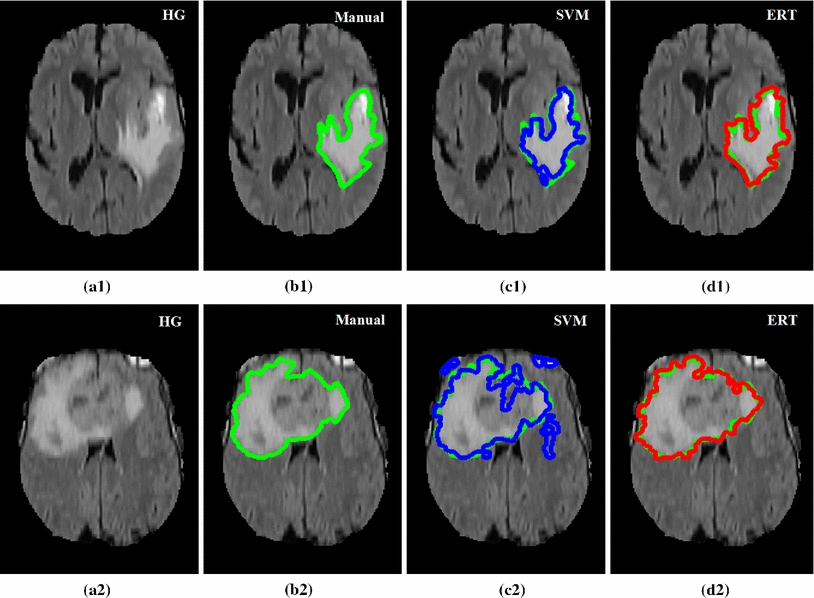
\includegraphics[width=10cm]{images/brain_segmentation.jpg}
\end{figure}

On other problems like finding and segmenting brain tumors on MRI images, medical professionals do not only look at the exact region where a tumor resides, but also at other regions of the brain. On the upper row of the scan above it is cleary visible that the tumor on the right side is extending the space used for the right half of the brain, and therefore many brain features are not symmetrical any longer. A neural network trained on this task should also use these cues to correctly segment the tumors. 

The main goal of this thesis is to provide such a tool by modifying existing interpretability methods to work on image segmentation.

\section{Planning}
All steps described here are prerequisites for the next step if not marked otherwise.

\subsection{NIH Chest X-ray}
To 



Purpose: Run some methods on a simpler dataset.
What is the dataset?
Used to figure out which methods work and can be used from PyTorch.
Use a basic image classificiation problem from the mediacal imaging field to evaluate methods.
\begin{itemize}
    \item Use the NIH chest x-ray dataset
    \item Learn a standard architecture for image classification on the model using PyTorch (e.g. Inception, ResNet)
    \item Apply methods on the output of the network
\end{itemize}


Goals
\begin{itemize}
    \item Determine which methods are directly usable with a PyTorch model or require low porting effort
    \item Determine which methods are independent of the used network architecture (methods that view the model as a black box)
    \item Find out how the output of the model looks like and (optionally) check with a medical professional which output they think would be most helpful
\end{itemize}


\subsection{Brain tumors}
Do built the methods to interpret image segmentation tasks, we need a real world task. Brain tumor segmentation is an interesting problem in the medical image field. Segmenting brain tumors manually is a tedious process, because MRI machines generate many slices of brain which then have to be looked at one by one. Automating the process with machine learning will give medical professionals more time to do other tasks and also gives them more confidence in their manual work when supported by an automated model.

To build a working machine learning model, some medical background is required. We will investigate what types of brain tumors exits, how do they look like on a scan and what scanner types exists (MRI/PET/CT). We also investigate how a tumor looks like on a specific scanner type.

\subsection{The BraTS dataset}
\begin{itemize}
    \item What scanner is used and what tumor types are detected?
    \item What data format is used to save the scans?
    \item In what format is the labeling saved?
    \item Build a loader for the dataset
    \item Display some scans
    \item Dataset: BraTS, extract 2D slices
    \item Do NOT use slice from same head in training \& validation set (they look nearly the same) 4 different labels, representing 4 different sizes of a tumor
    \item Merge innermost 2 layers into one
    \item an image has 4 black/white channels, use them as separate channels
\end{itemize}

\subsection{Model for the BraTS dataset}
A widely used architecture for segmentation (especially in the medical imaging field) is the UNet architecture

\begin{itemize}
    \item Research current state of the art networks for image segmentation
    \item Investigate U-Net architectures
    \item Build and train network for the BraTS dataset in PyTorch based on an existing architecture
    \item Investigate and if necessary/helpful implement data augmentation for the dataset
\end{itemize}


\subsection{RISE}
Randomized Input Sampling for Explanations (RISE) is a interpretability method that uses the model as a blackbox. It does not need to know anything about the underlying machine learning model, it only needs access to the input image and the probabilities of the output classes.

RISE generates a series of masks which get applied to the input image. The modified image is then run through the model and the changed probabilities of the output classes are recorded. From the probabilities of the different masks, a heatmap is generated which shows which parts of the image influence the correct classification of the image the most.

todo Challenge: RISE works with classificatin, how can we remodel it to use segmentation output
Blackbox model

\subsection{Other blackbox model methods (Optional}
There are other blackbox methods (e.g. LIME\cite{ribeiro2016should}) which work similar to RISE. If a successful method is found to apply RISE to image segmentation tasks, modifing these other methods to also for segmentation should not be a major problem.

A high quality solution with RISE has a higher priority than adding additional methods.

\subsection{Grad-CAM Method}




Example for a whitebox model. Whitebox idea: dynamic unet can use standard model arch (e.g. resnet), so we can use these on half the network => does it make any sense?
Many implementations for PyTorch, an example for a whitebox model. If we get this to work, other methods should be possible too.

Do these methods work when we do not have a class? Only a specific activation?

works on UNET!

Because this method is a whitebox model, it is independent of the implementation of the RISE model.


\subsection{Other whitebox model methods (Optional}
As described above, there are many whitebox model methods which can be applied to this problem.

\subsection{Library}
Build a library with a common interface for the implemented tools, so that all of them can be applied easily.
\begin{itemize}
    \item Write example programs for the library to use with PyTorch
    \item (Optional) Write example programs for the library to use with TensorFlow
    \item Write documentation how to use the library
    \item (Optional) Publish on conda
    \item (Optional) Publish on PyPI
    
\end{itemize}

\section{Infrastructure and technology}
This work will use the PyTorch\cite{paszke2017automatic} deep learning library. Most newer machine learning papers are written with PyTorch, because it is considered easier to learn and more powerful than Keras and PyTorch\cite{pytorchvstensorflow}.

Other machine learning libraries will be used on demand, for example:

\begin{tabular}{|p{3cm}|p{12.5cm}|}
    \hline
    \textbf{Library} & \textbf{Description} \\ \hline
    Scikit & Diverse kit of machine learning libraries \\ \hline
    Matplotlib & Library to generate graphs \\ \hline
    PIL/Pillow & Image manipulation library \\ \hline
    NumPy & Matrix manipulation library \\ \hline
    pandas & Dataframe library \\ \hline
    torchvision & PyTorch extension for computer vision problems. Contains models for common architectures and pretrained parameters for these networks. Also contains tools for data augmentation. \\ \hline
\end{tabular}

The development of the system will take place inside Jupyter notebooks. Jupyter notebooks allow a very fast test and development cycle. The notebook server will be running on a powerful desktop computer of the author which is exposed to the internet, so the computational power is always available independent of the work location.

In addition, the GPU servers from the Berner Fachhochschule (NVIDIA DGX-1, 4x Tesla V100) and from the Institute for Surgical Technology and Biomechanics of the Universität Bern (Unknown number and type of GPUs) are available. Because the setup cost to use these servers is quite high, the usage of these systems is optional and time will only be invested if the learning speedup is worth the additional setup time.

\section{GANT Chart}
